\documentclass[11pt, a4paper]{article}
\usepackage[utf8]{inputenc}
\usepackage[english,russian]{babel}

\usepackage{a4wide}
\usepackage{graphicx}
\usepackage{caption}
\usepackage{amssymb}
\usepackage{amsmath}
\usepackage{mathrsfs}
\usepackage{euscript}
\usepackage{theorem}
\usepackage{graphicx}
\usepackage{subfig}
\usepackage{caption}
\usepackage{color}
\usepackage{bm}
\usepackage{tabularx}
\usepackage{adjustbox}

\usepackage{rotating}

\DeclareMathOperator*{\argmax}{arg\,max}
\DeclareMathOperator*{\argmin}{arg\,min}

\newcommand*{\No}{No.}
\begin{document}
\title{\bf Attention для апроксимации временных рядов}
\date{}
\author{}
\maketitle

\section{Некоторое введение}
Под временным рядом будет предполагать набор упорядоченных точек, которые получены путем наблюдения за некоторым непрерывным процессом с некоторой фиксированной частотой.

\section{Модель seq2seq и Attention}

\begin{figure}[h!]\center
\subfloat[Описаниие seq2seq]{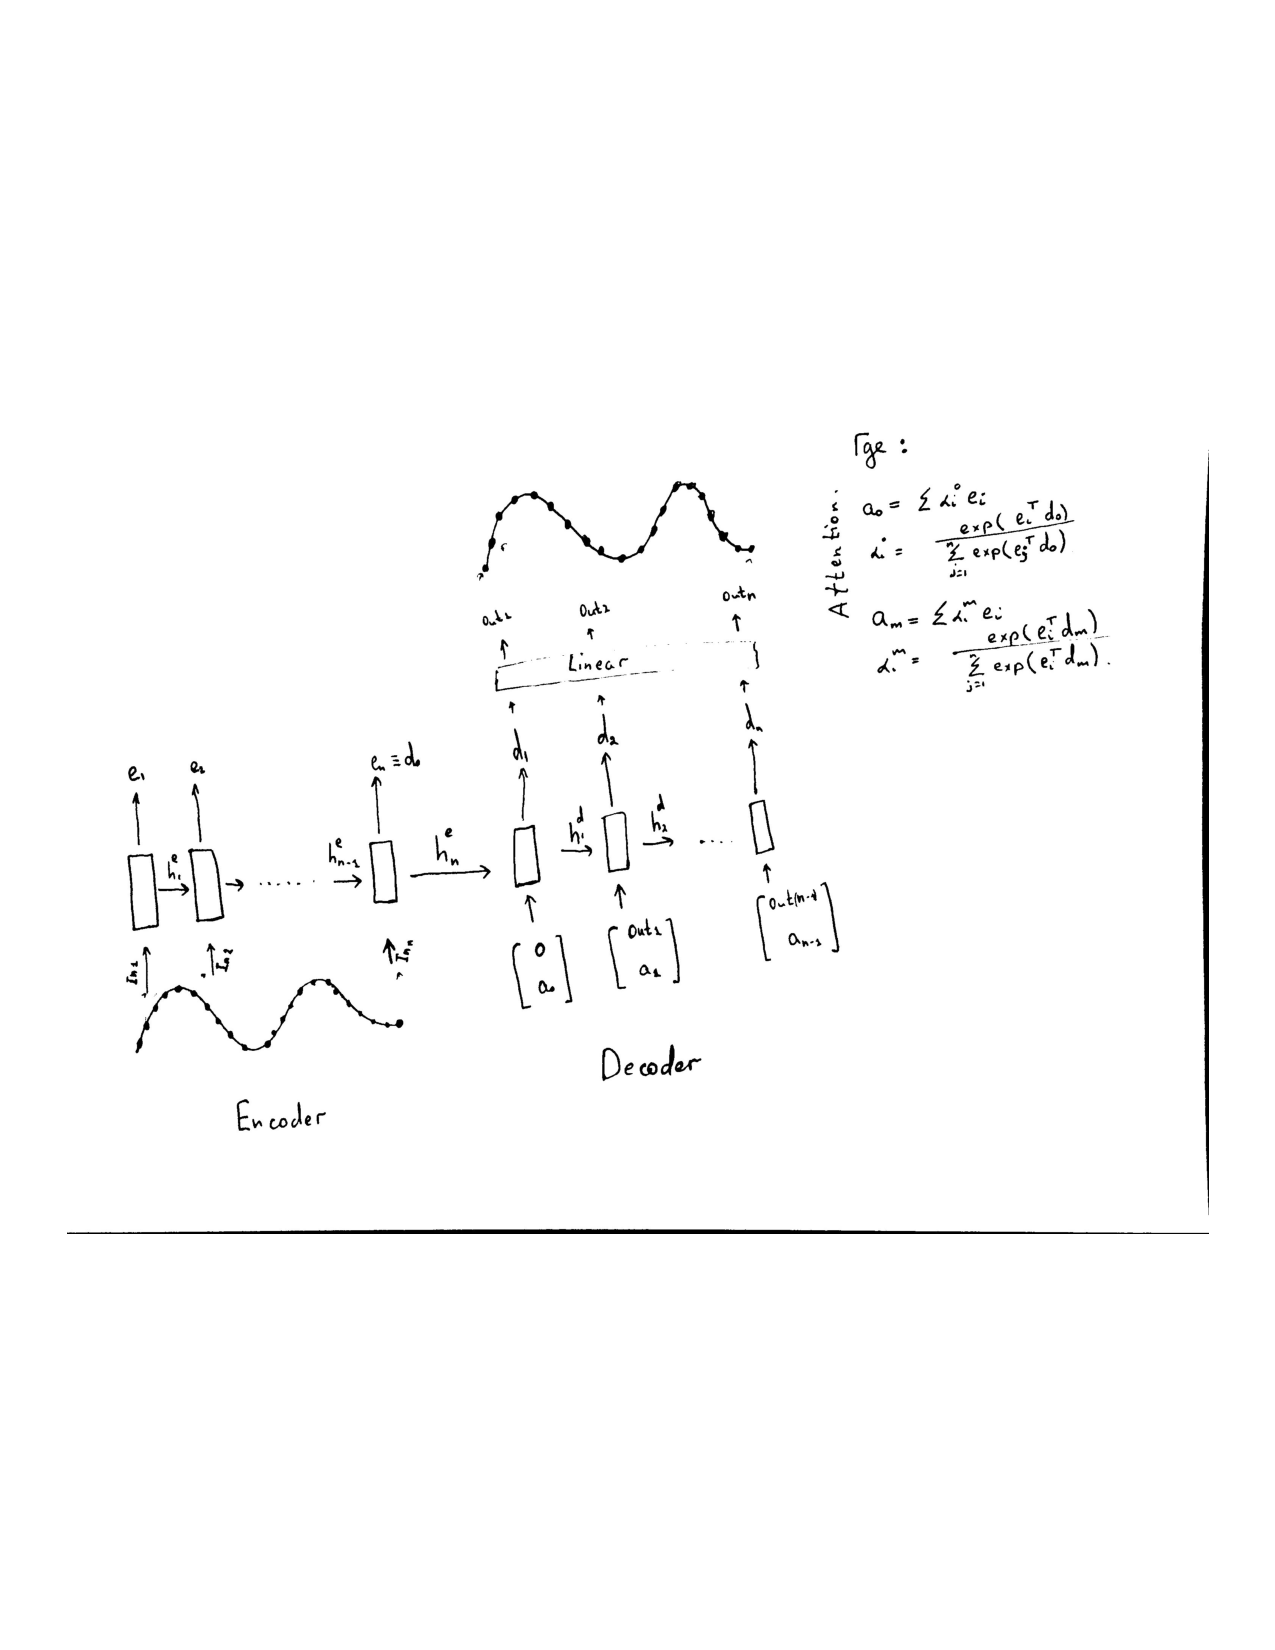
\includegraphics[width=0.5\textwidth]{figures/img1.pdf}\label{fig1}}
\subfloat[Описаниие предполагаемых результатов]{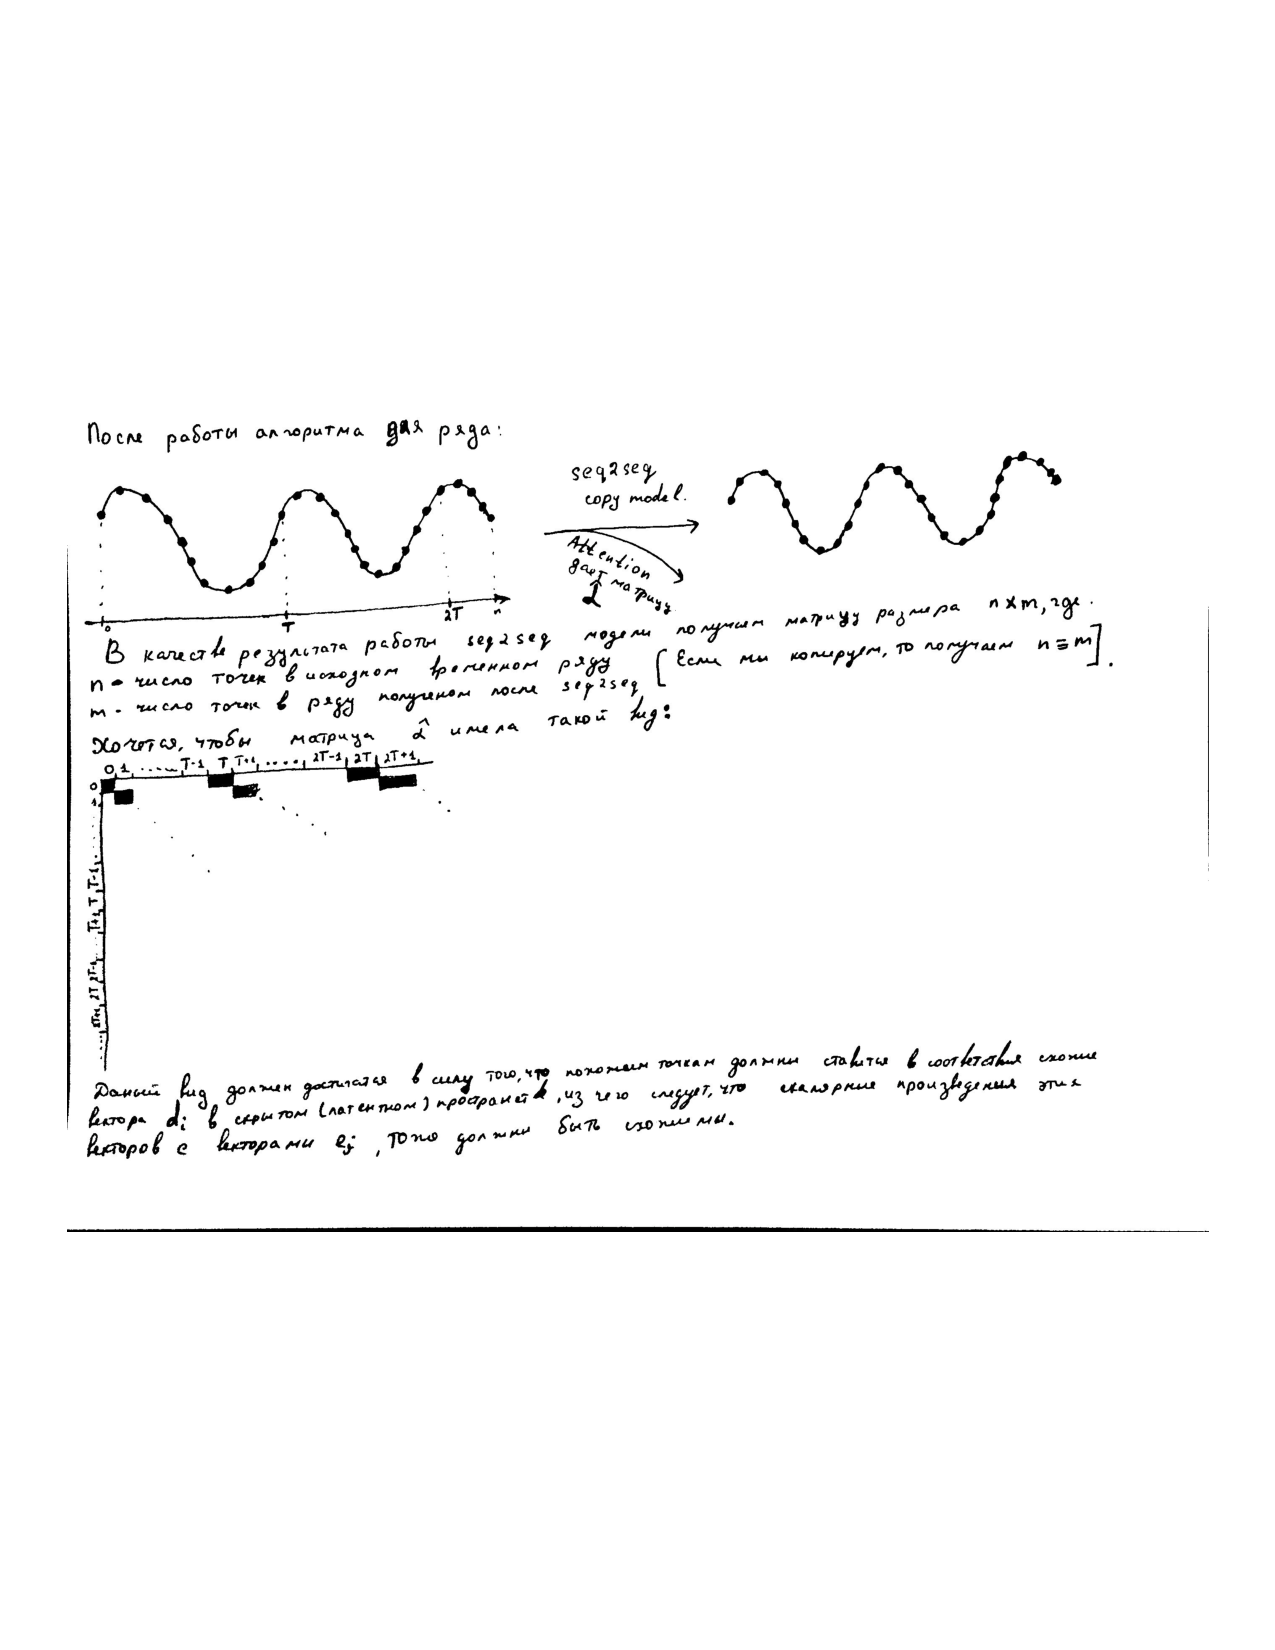
\includegraphics[width=0.5\textwidth]{figures/img2.pdf}\label{fig2}}
\caption{Основные сведения об seq2seq + Attention}
\end{figure}

Используем LSTM с простейшим Attention без дополнительных параметров. Пример, принцепа работы seq2seq c Attention показан на рис.~\ref{fig1}.

\section{Предположения}
Введя предположения о том, что скрытые вектора LSTM имеет похожие вектора для похожих кусков временного ряда можно предположить, что матрица Attention будет иметь вид показан на рис.~\ref{fig2}. Под матрицей Attention подрозумевается матрица размера $n\times m$, где $n, m$ --- длины входного и выходного сигналов соответственно, в ячейках которой показан уровень схожести (либо можно сказать уровень зависимости) между куском временного ряда на выходе и куском временного ряда на входе.

\section{Проблемы}
Предлагается использовать seq2seq, который просто копирует временной ряд. В этом методе есть ряд вопросов.
\begin{itemize}
    \item Первый косяк состоит в том, что если мы учим копировать временной ряд, и берем слишком сложный Attention с большим количеством параметров, то он начинает переобучатся, и в итоге получается матрица Attention диагональной. Это следует из того, что модель начинает просто учить друг за другом числа. Поэтому предлагается использовать просто скалярное произведение векторов (самую простую модель Attention, Dot метрика из~\ref{tab1}).
    
    \item Даже если взять простую модель Attention, все равно можно получить диагональную матрицу Attention, если мы просто будем копировать временной ряд, поэтому предлагается не просто учить все ряды из обучающего множества рядов, а на вход Encoder'а давать некоторый кусок (например из 100 сигналов ряда дать только первые 20 сигналов), и сравнивать как Decoder восстановит весь сигнал. Данный дополнительный финт немного улучшает качество.
    
    \item Второй вопрос состоит в том, что нужно придумать на каких данных учить данную модель (нужно подумать над тем какие сигналы давать на вход для копирования). Этот вопрос возникает в синтетических данных, но и в реальных данных. Я думаю, что можно модель учить не только на реальных данных, а и на синтетических, но для этого нужно придумать максимально правдоподобный сигнал акселерометра.
    
\end{itemize}

\begin{table}[h!]
\begin{center}
\caption{Описание разных Attention}
\label{tab1}
\begin{tabular}{|c|c|}
\hline
	Type & formula\\
	\hline
	Additive& $score_{i,j}~=~\tanh\left(\textbf{W}_e\textbf{e}_i+\textbf{W}_d\textbf{d}_j\right)$\\
	\hline
	Dot& $score_{i,j}~=~\textbf{e}_i^{\mathsf{T}}\textbf{d}_j$\\
	\hline
	General& $score_{i,j}~=~\textbf{e}_i^{\mathsf{T}}\textbf{W}\textbf{d}_j$\\
\hline
\end{tabular}

\end{center}
\end{table}

\section{Эксперимент}
\subsection{Эксперимент с простыми переодическими структурами}

\begin{figure}[h!t]\center
\subfloat[$sin(x)$]{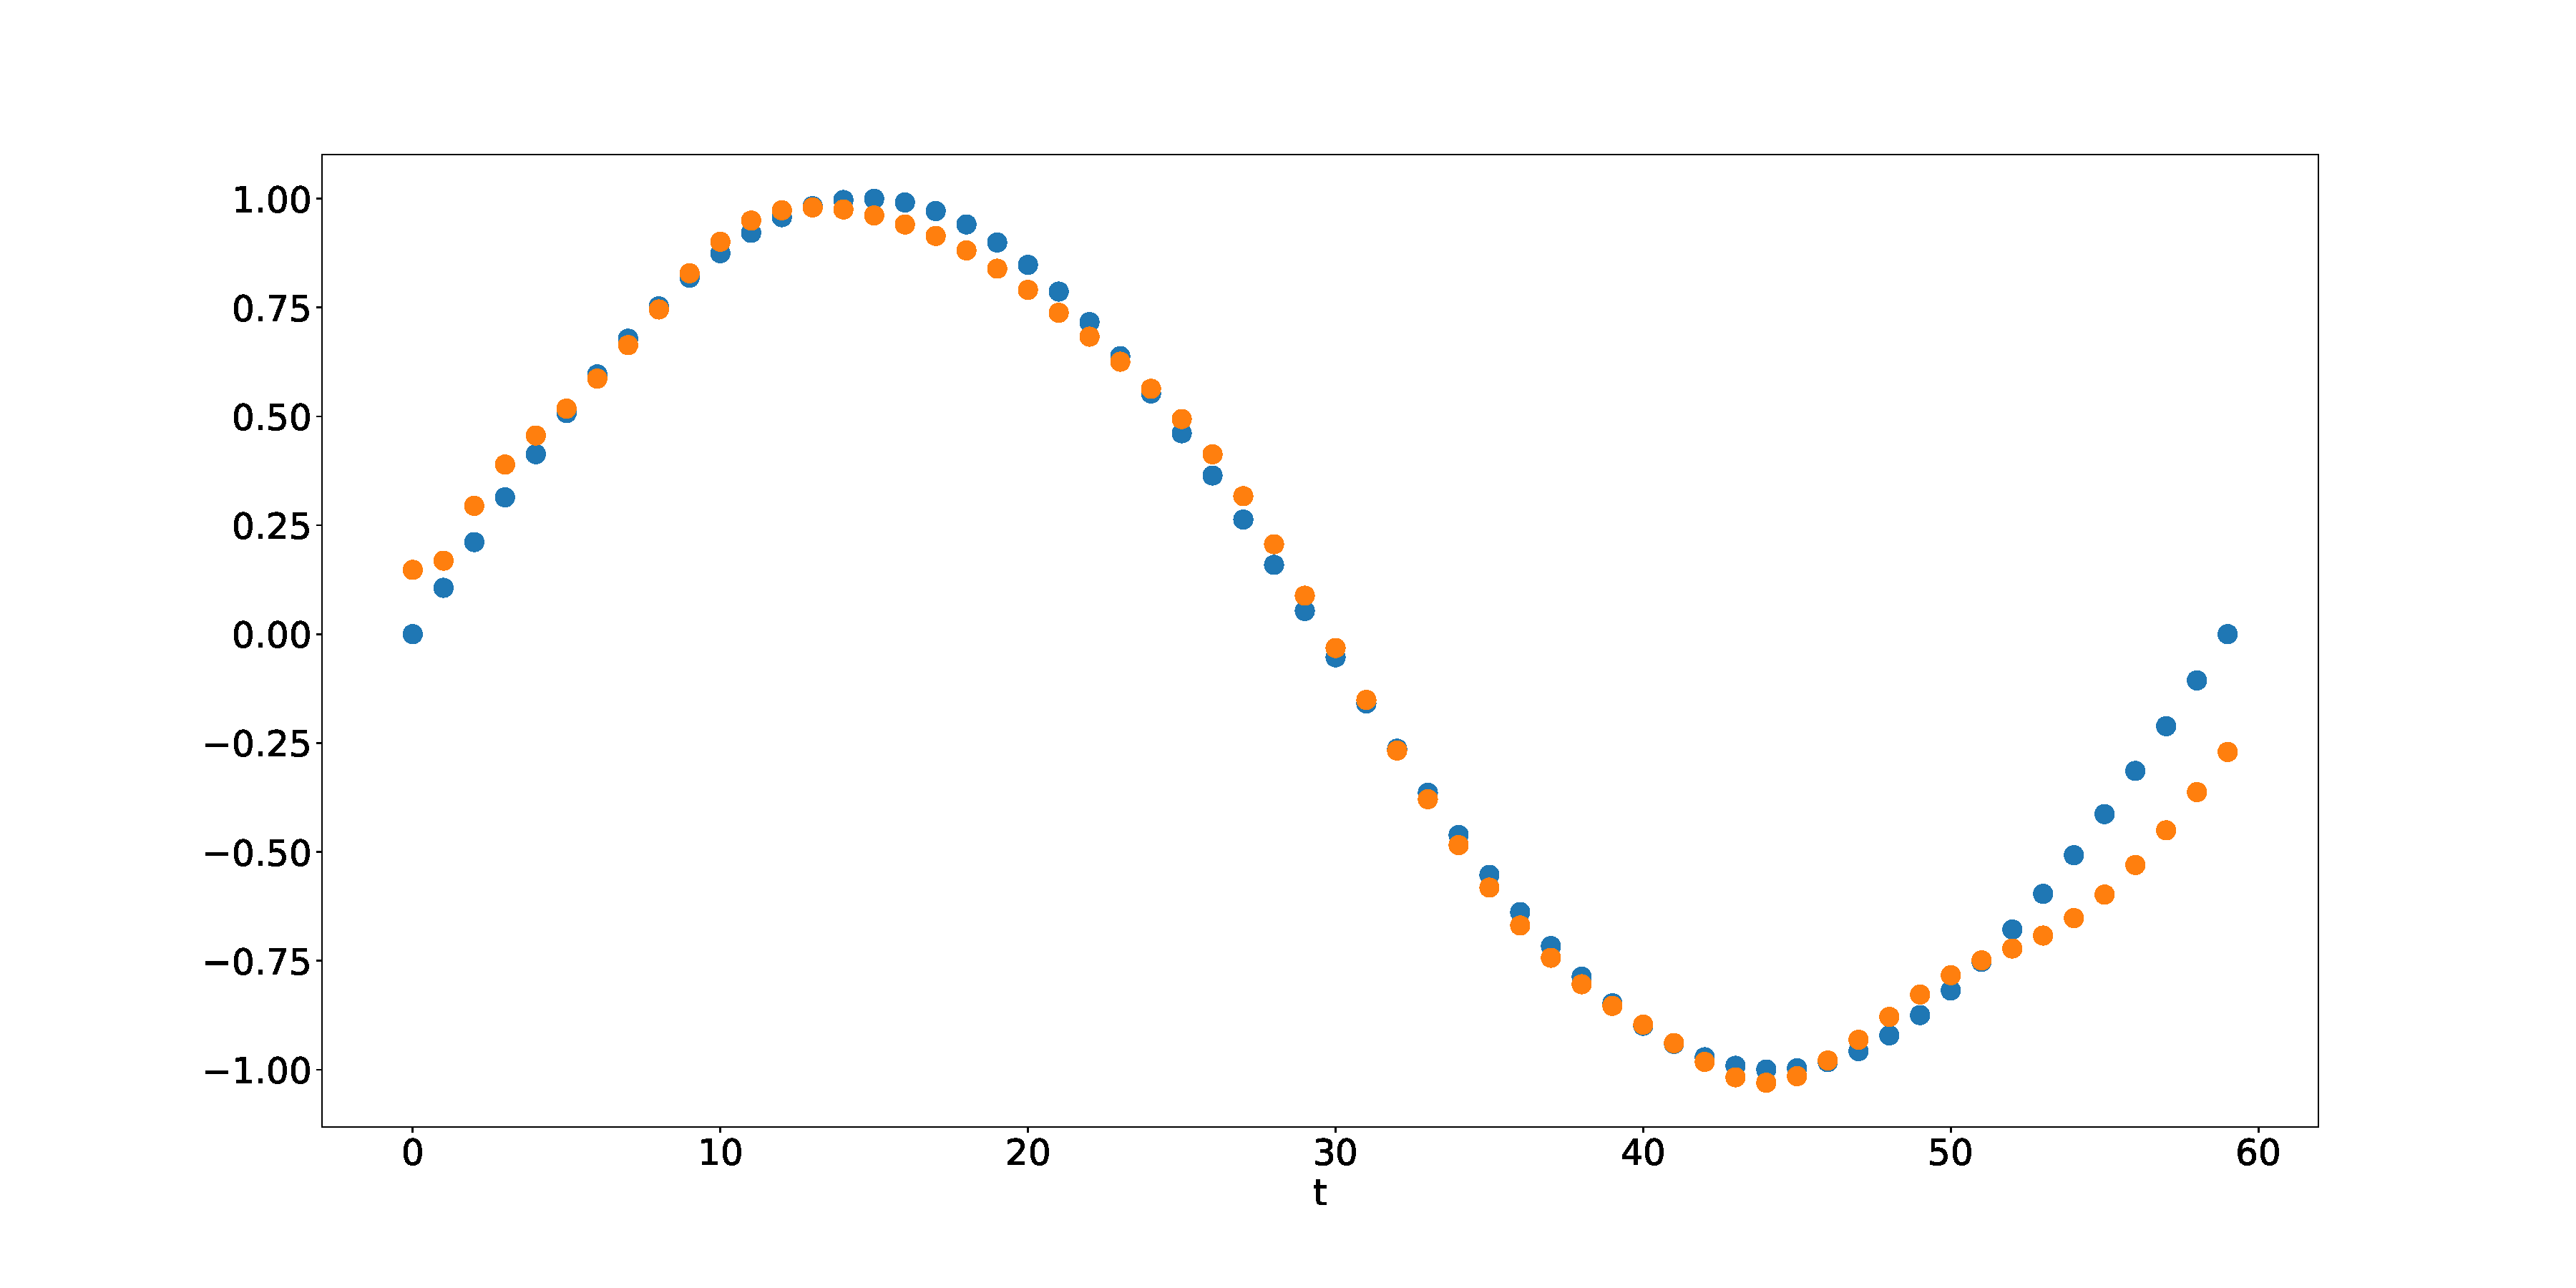
\includegraphics[width=0.5\textwidth]{figures/TimeSeries1.pdf}}
\subfloat[$sin(x)$]{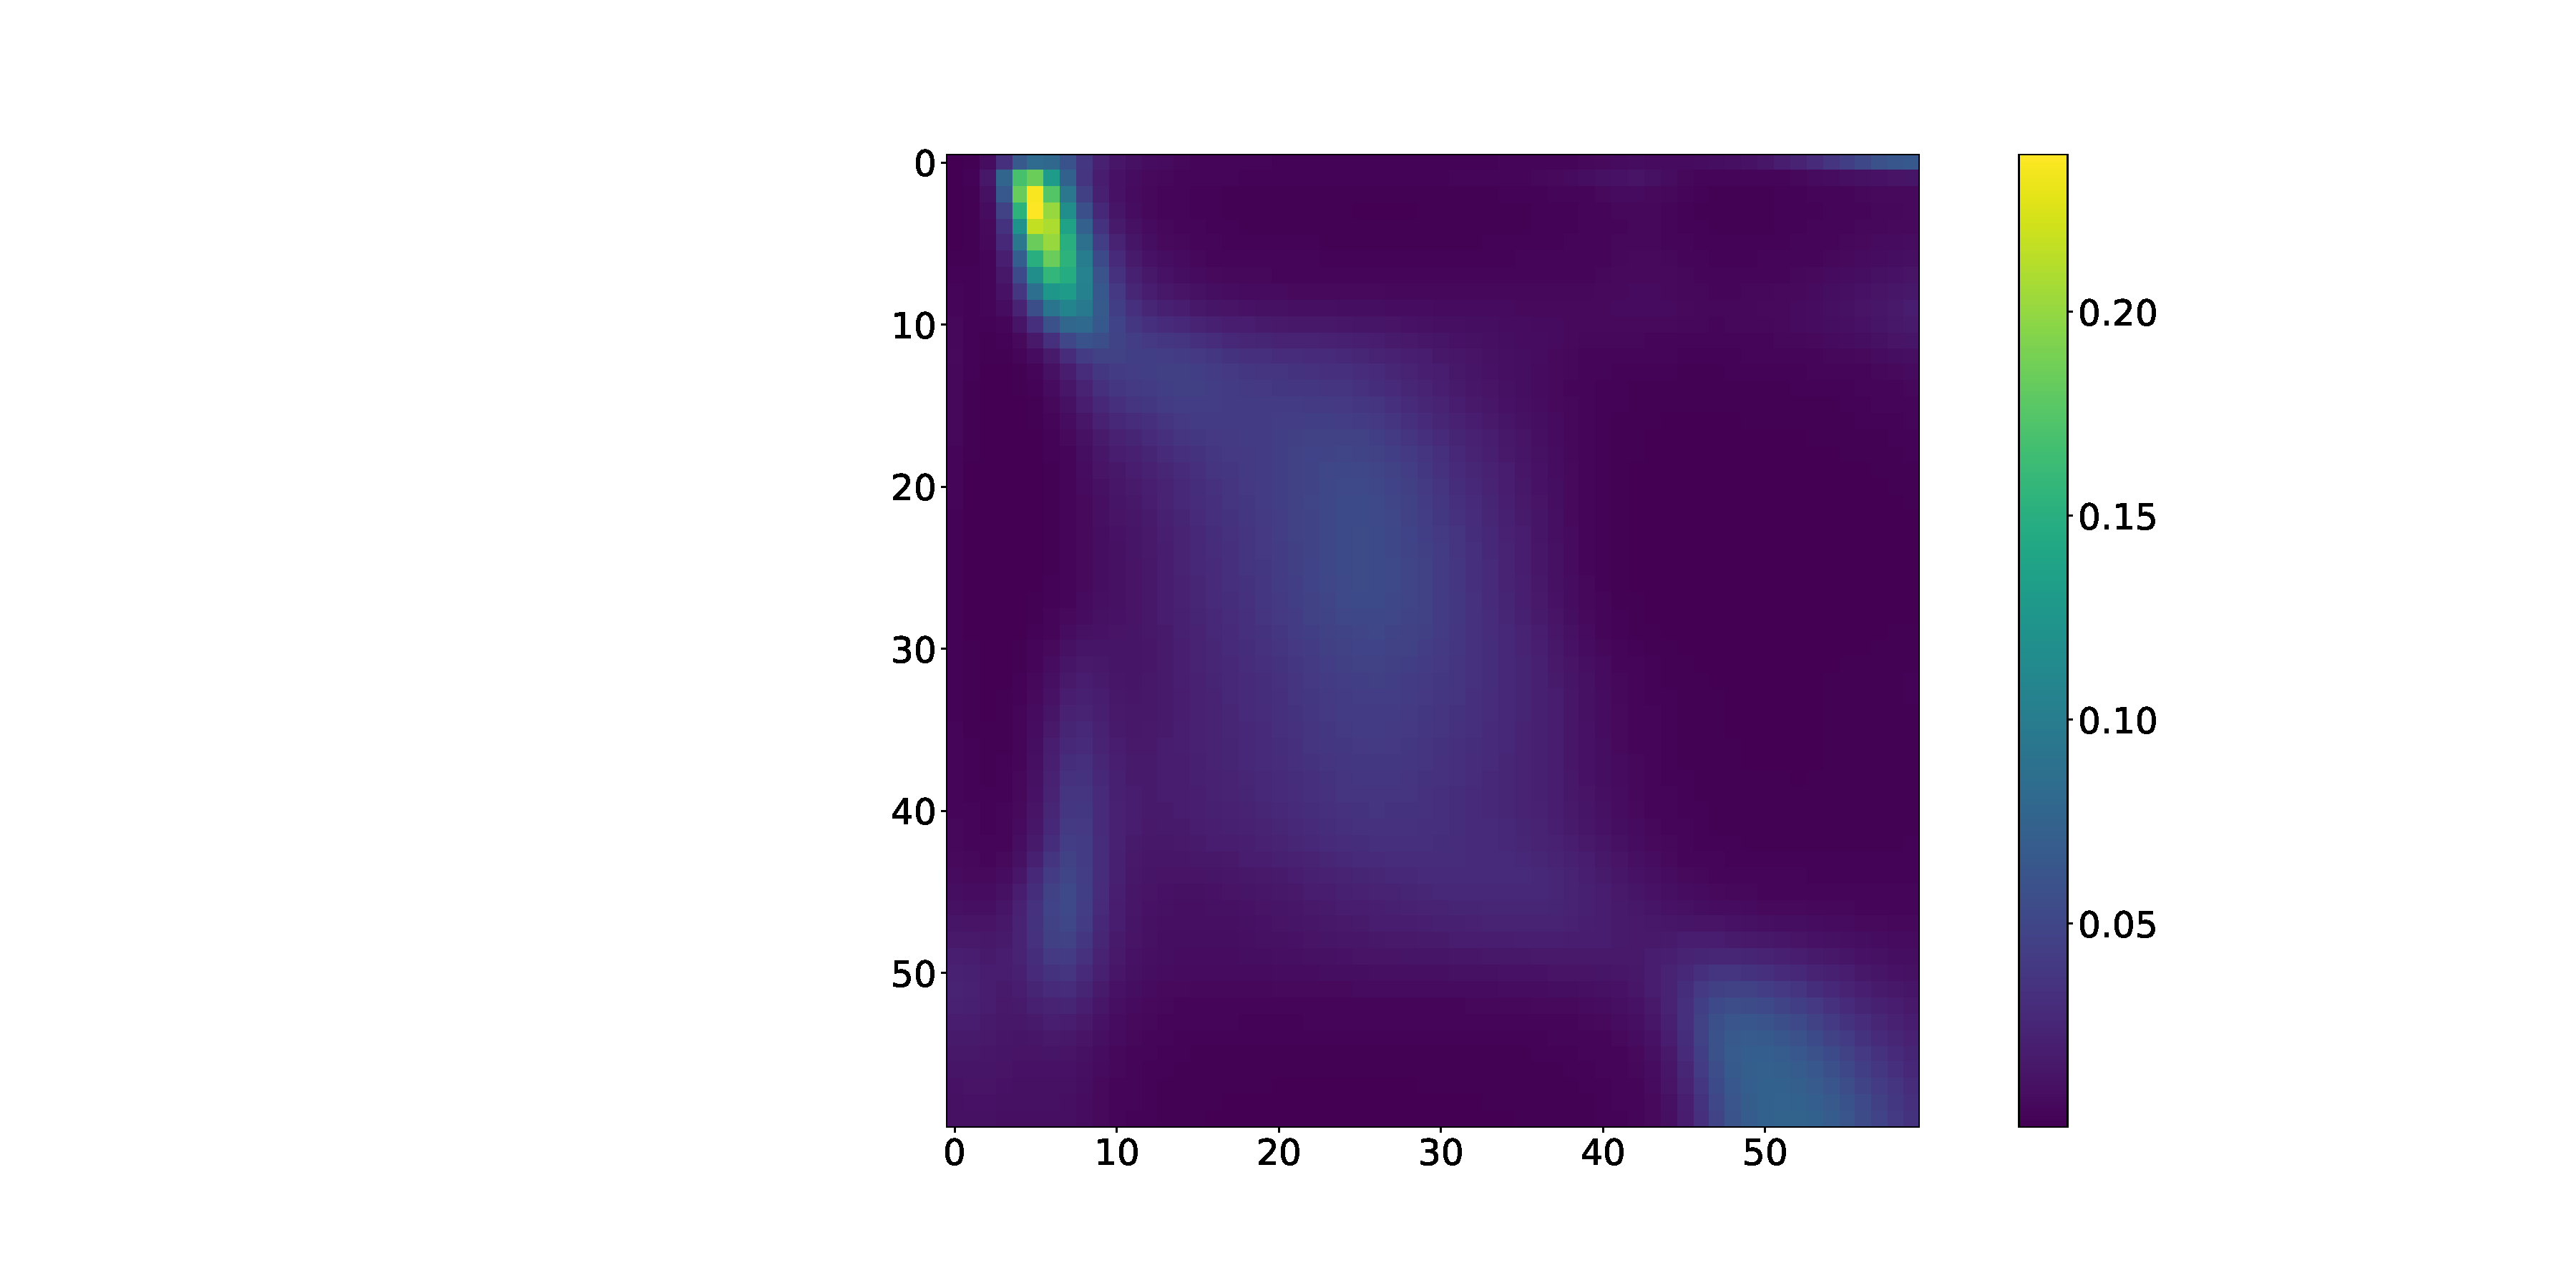
\includegraphics[width=0.5\textwidth]{figures/Attention1.pdf}}\\
\subfloat[$sin(2x)$]{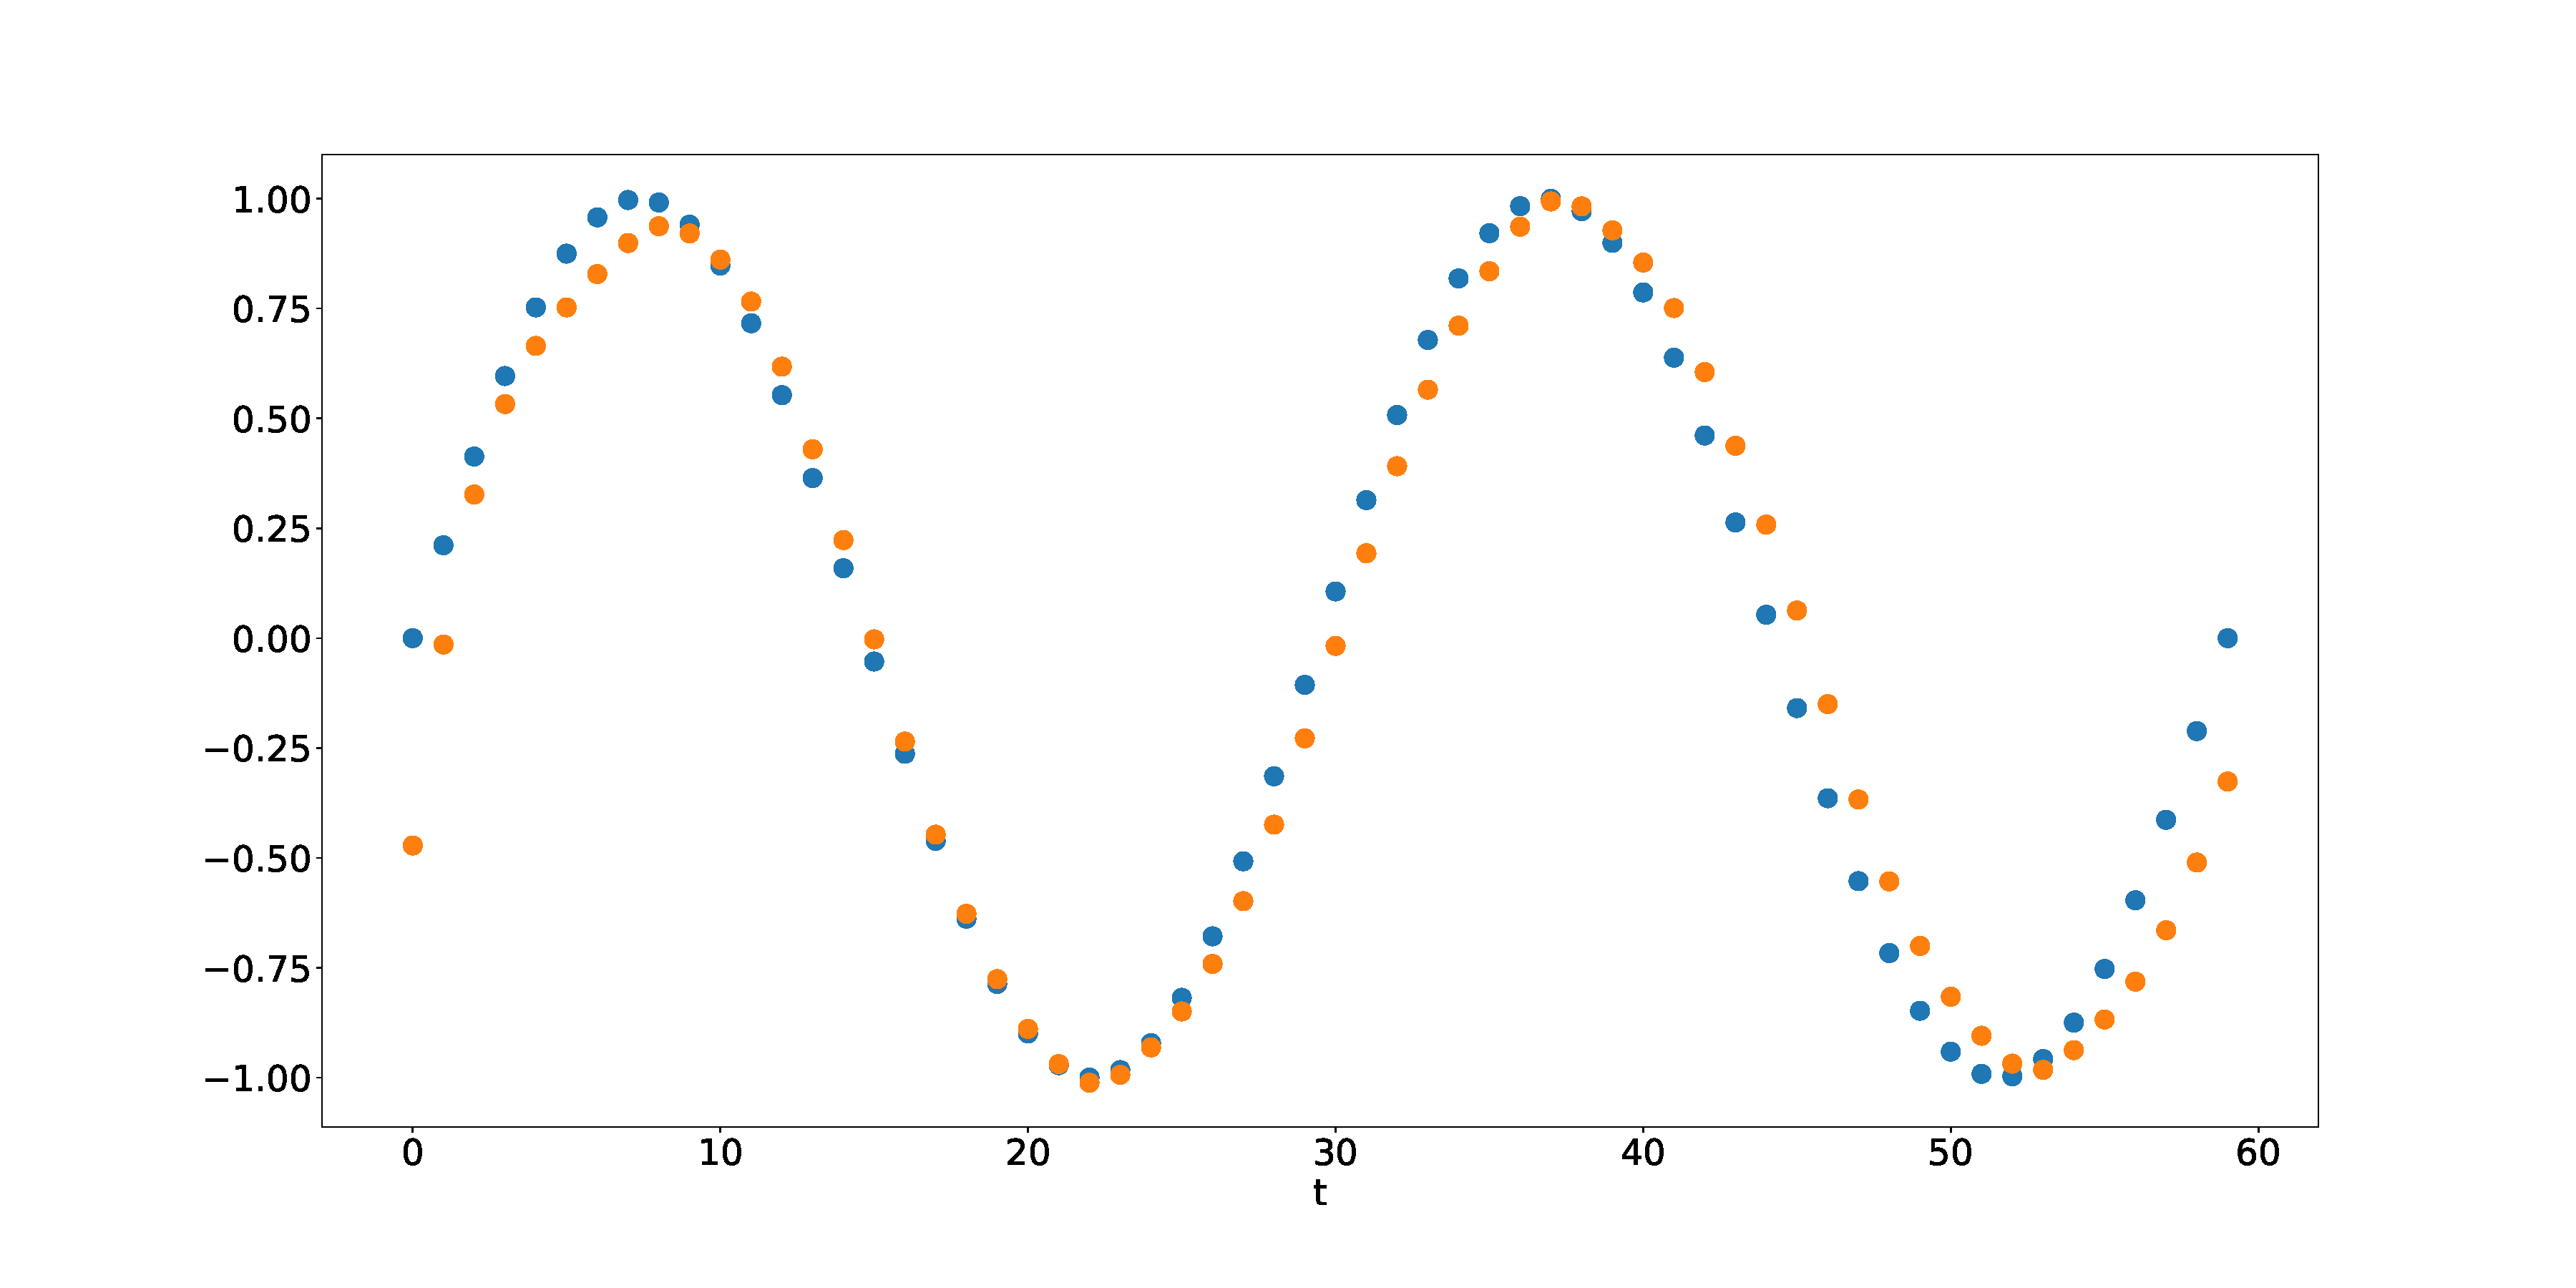
\includegraphics[width=0.5\textwidth]{figures/TimeSeries2.pdf}}
\subfloat[$sin(2x)$]{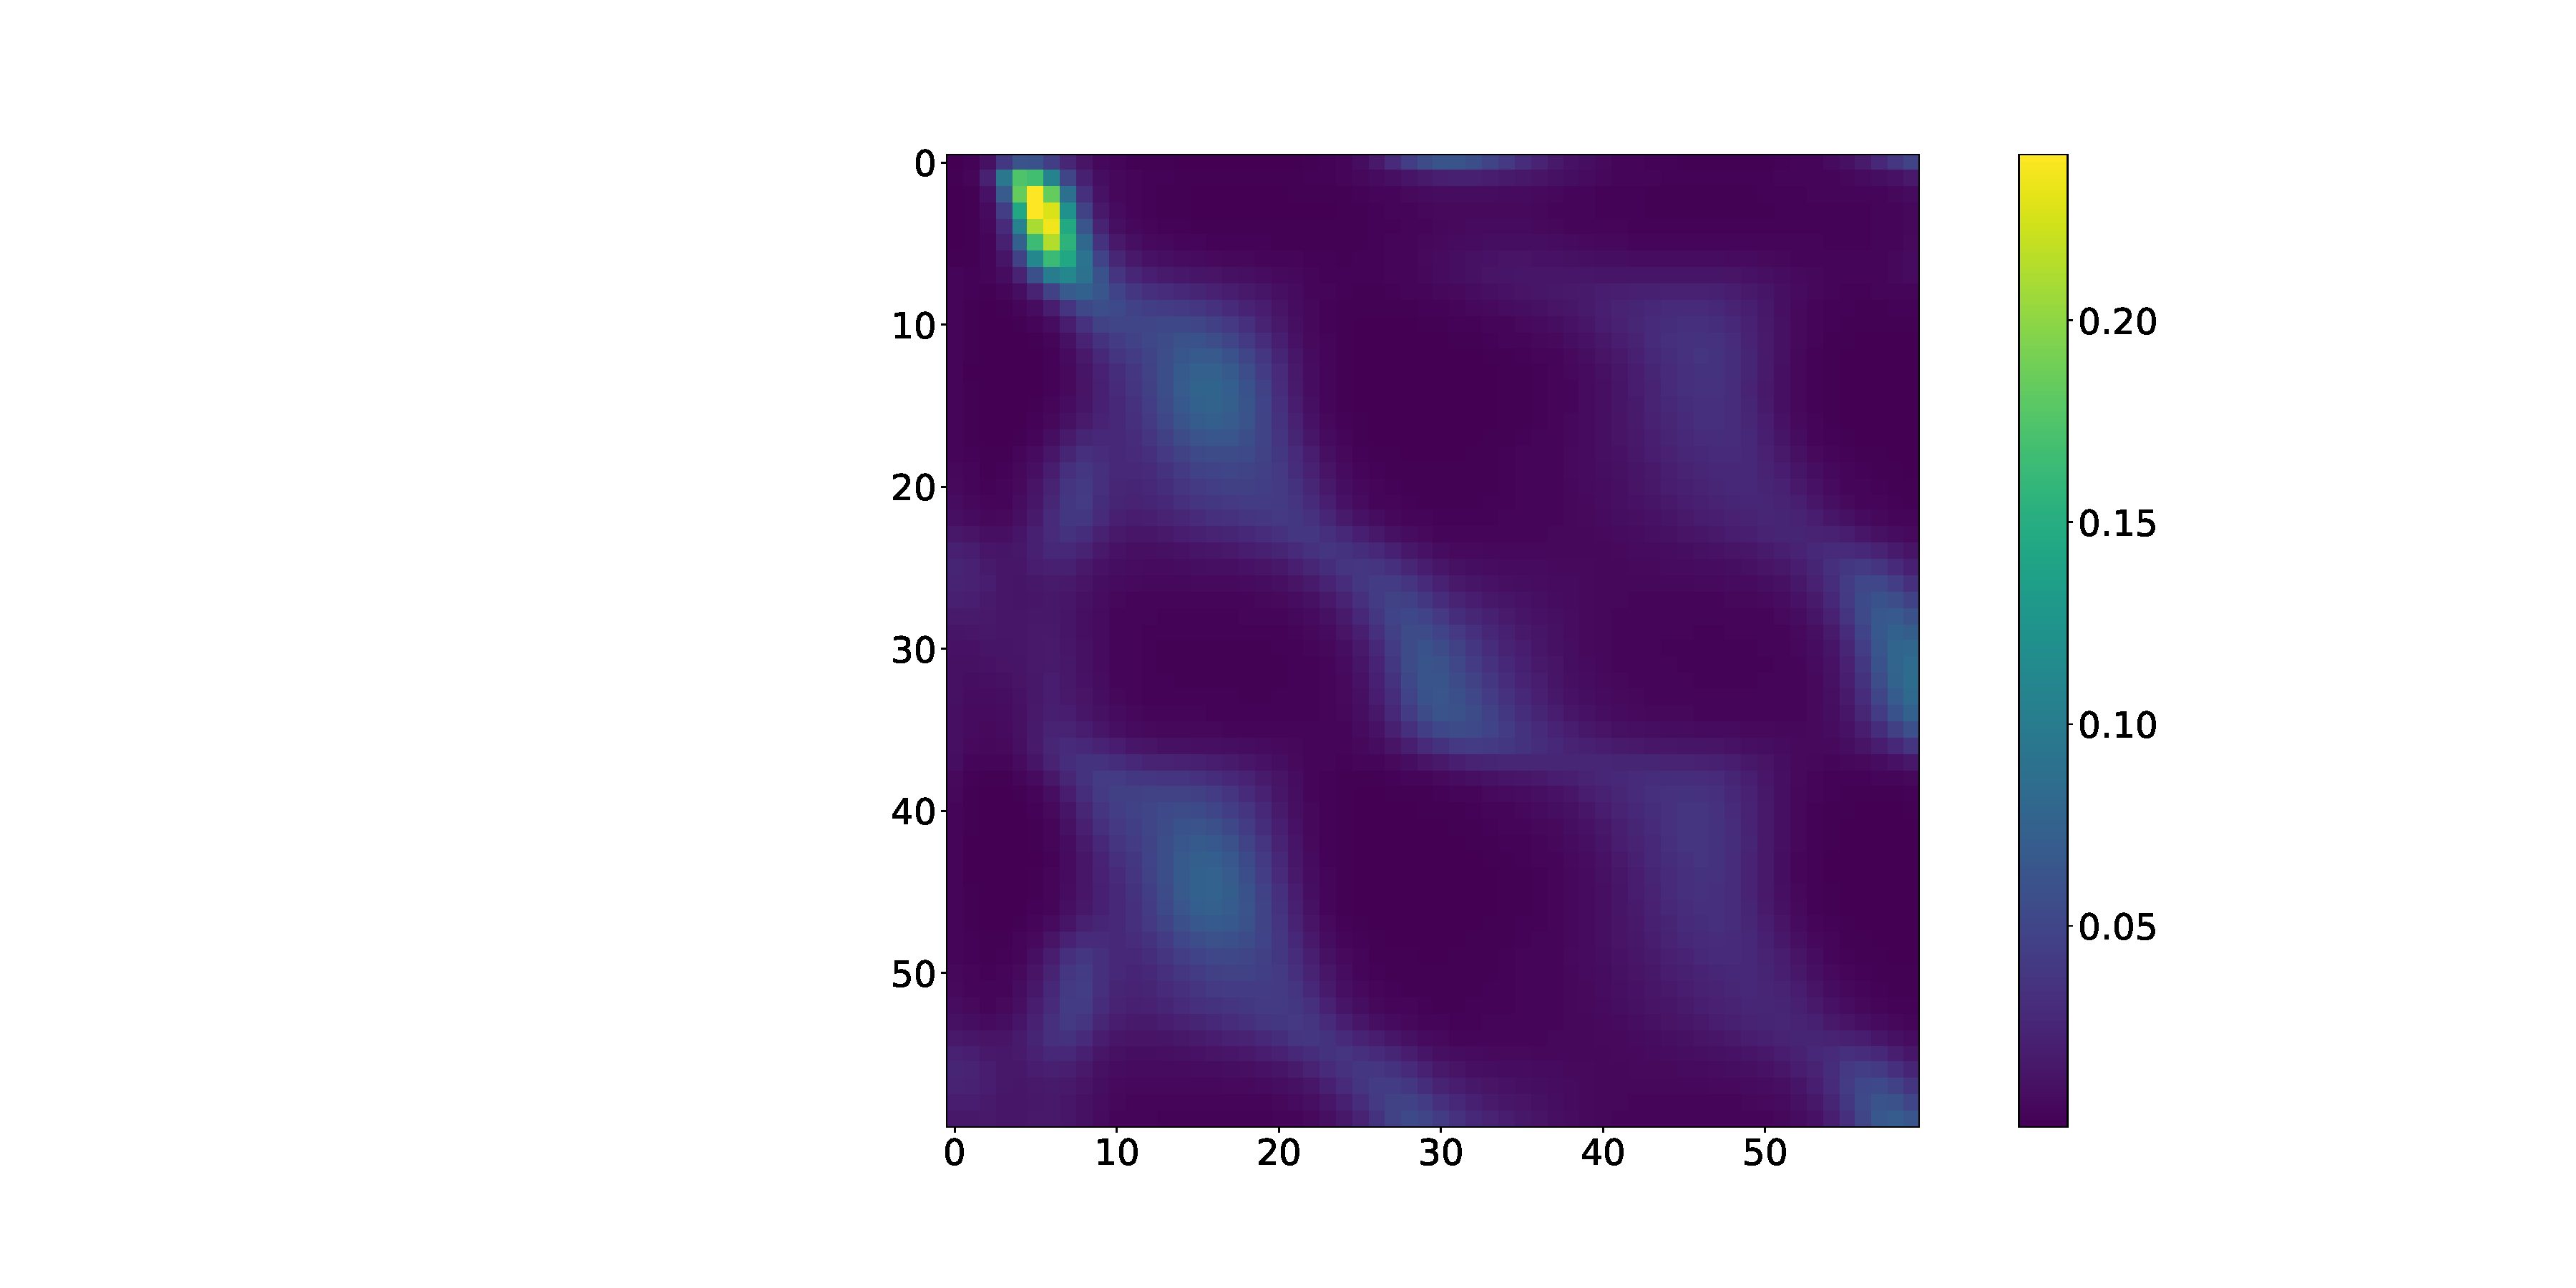
\includegraphics[width=0.5\textwidth]{figures/Attention2.pdf}}\\
\subfloat[$sin(8x)$]{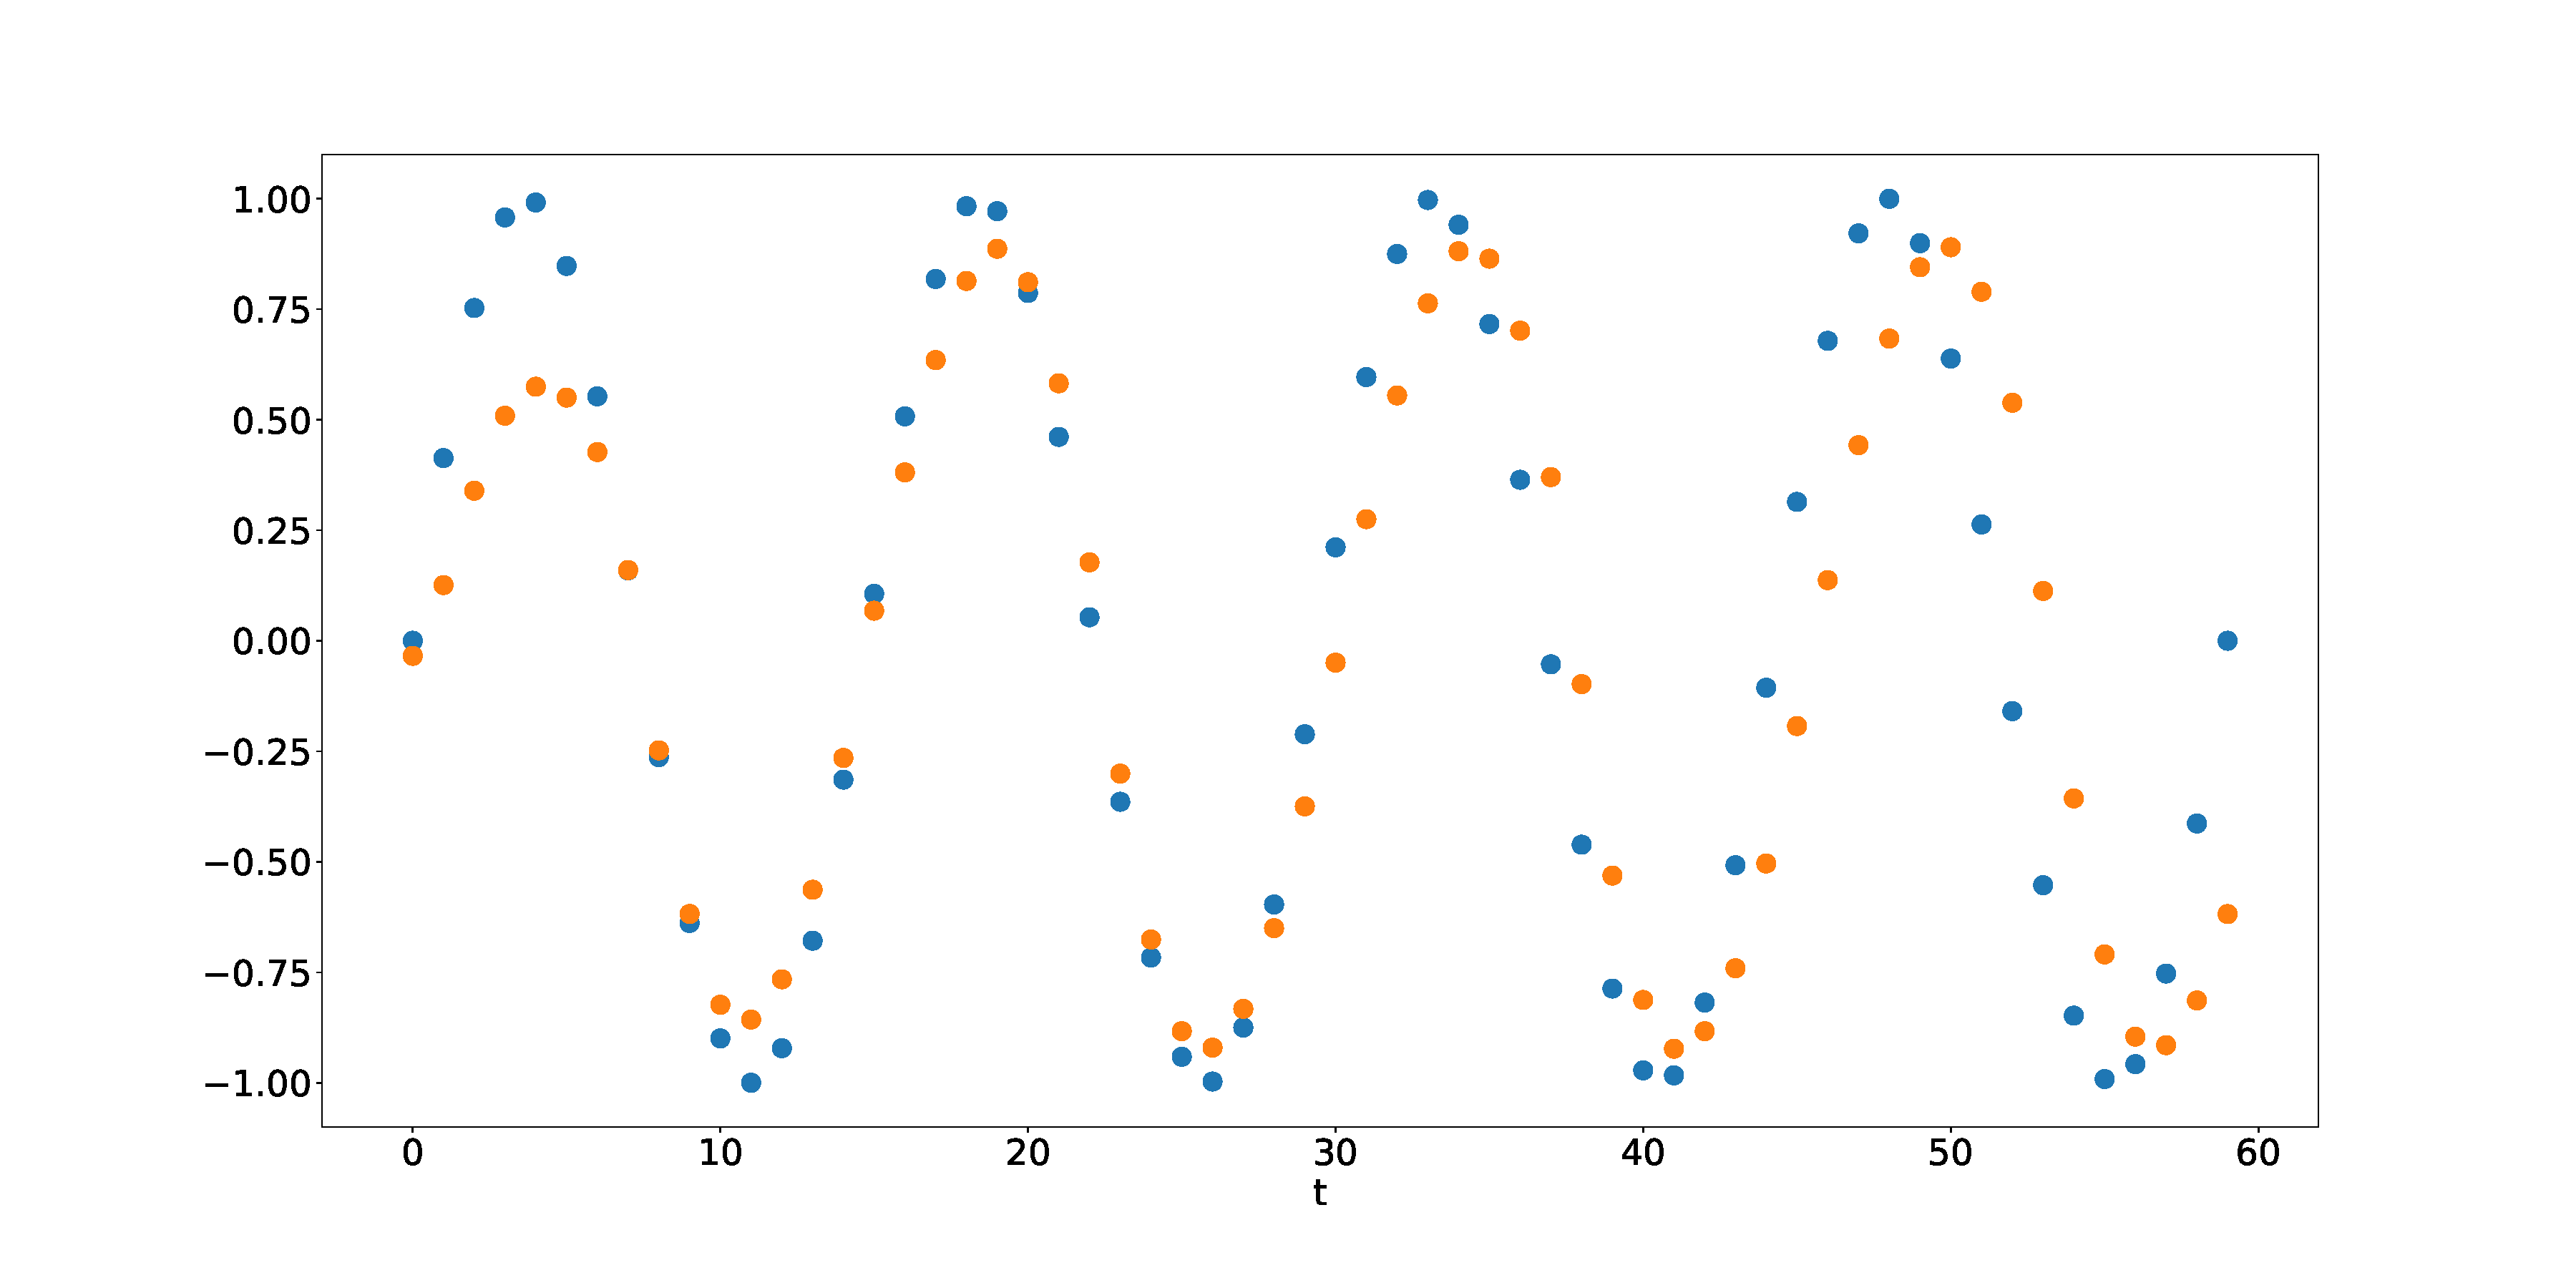
\includegraphics[width=0.5\textwidth]{figures/TimeSeries3.pdf}}
\subfloat[$sin(8x)$]{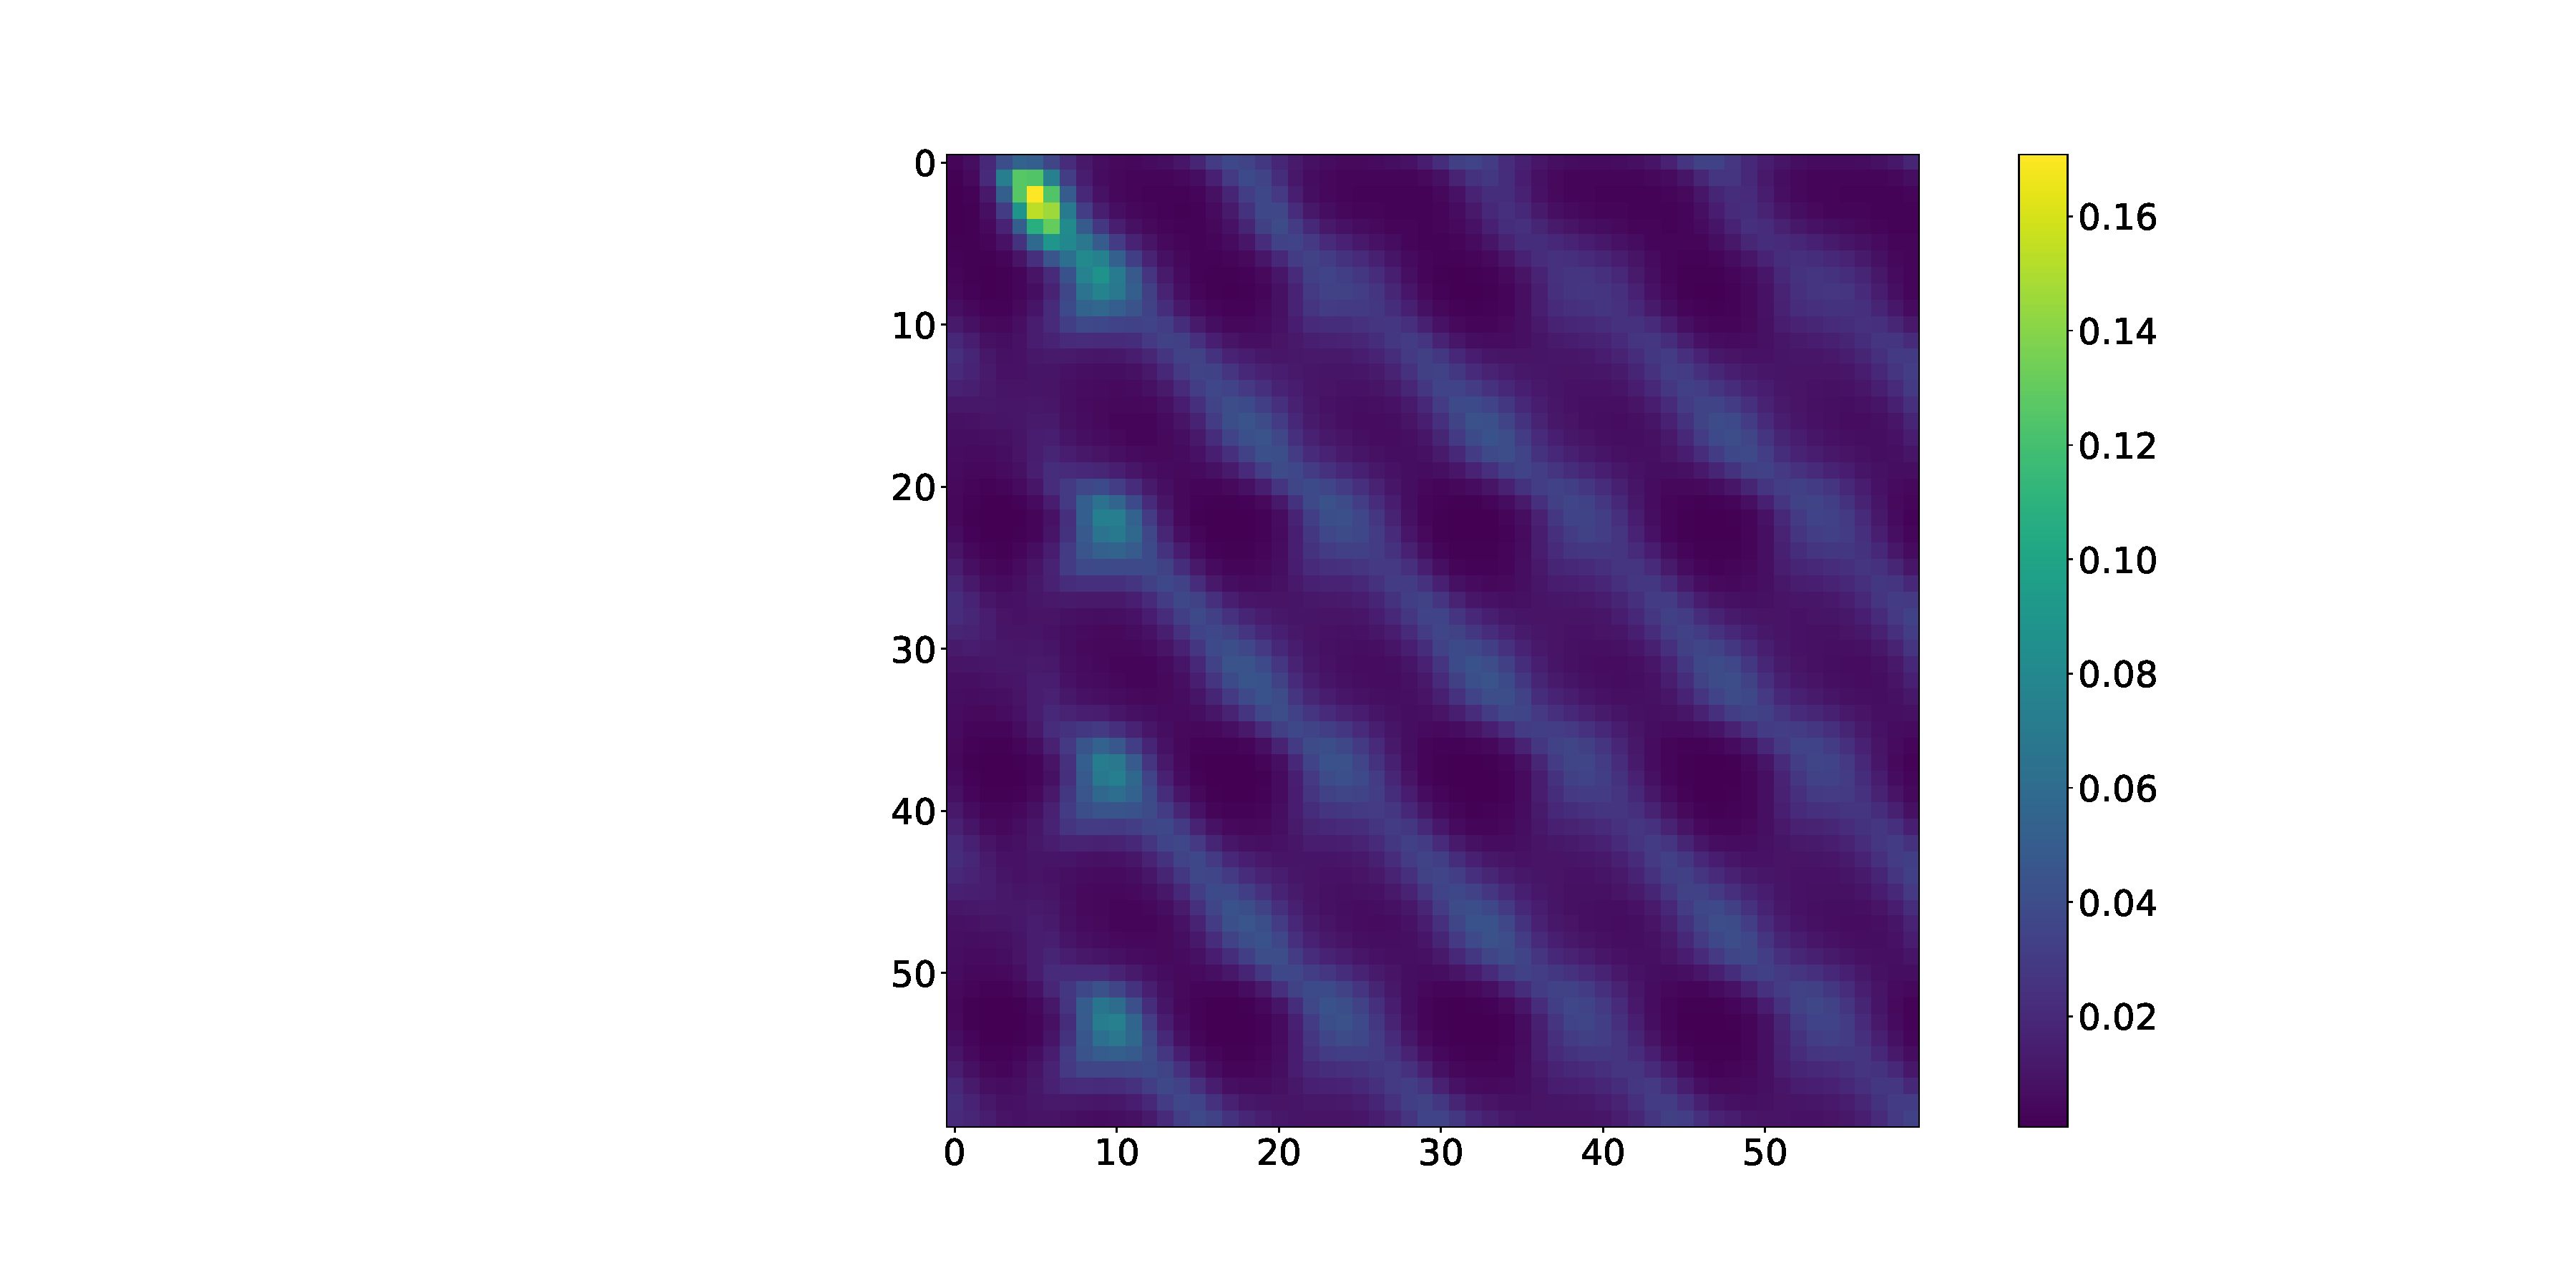
\includegraphics[width=0.5\textwidth]{figures/Attention3.pdf}}\\

\caption{Результаты для модели с рис.~\ref{fig1}}
\label{fig3}
\end{figure}



Пусть модель обучена на синусоидальных сигналах с произвольной частотой, произвольной амплитудой и произвольной начальной фазой. Как видно из результатов на рис.~\ref{fig3}, предположение о виде матрицы Attention подтверждается. На рис~\ref{fig3} показано как меняется вид матрицы Attention в зависимости от частоты синуса. Видно что количество диагоналей в матрице Attention соответствует частоте синусоидального сигнала.

\subsection{Эксперимент со сложными переодическими структурами}


\end{document}

